\chapter{Micro-location}
\label{cha:microlocation}

% Motivation

The primary motivation for providing an ultimate solution to the micro-location problem is enabling a new wave of mobile---possibly artificially intelligent---applications. Possible uses of micro-location are unimaginably limitless (by analogy, it suffices to browse through endless lists of mobile applications for the ``GPS'' query in any application store). Below, there are some of the most quick and straightforward ideas.

\begin{itemize}
	\item Museums were the main use case when this project came to life, as they are the most obvious one. One can imagine walking through Louvre with their own smartphone describing all exhibits \emph{interactively}! Almost like walking with one's own rented guide. And with the advances in artificial intellect, this experience might start to become more and more like it.
	
	\item Big shopping centers and malls could benefit greatly from micro-location capabilities. Users (customers) would no longer got lost. (Or, arguably, is it to the center owners' benefit that they got lost?) Especially so, if micro-location data was used with customer profiling, machine-learning what they might want to buy and why.
	
	\item Large building of some public (to a certain extent) services, like government buildings, campuses, big office buildings, enormous hospitals\ldots While their employees may know arrangements and purposes perfectly, it's not that clear to customers, citizens, students, people who visit these buildings for the first time in their lives.
	
	\item Another category of public space is various venues related to transportation of---mainly---people. Airport, train stations buried deep underground might overwhelm some, especially if there are only five more minutes left to get on one's next line. Precise navigation accompanying the user can be imagined to be at least a blessing.

	\item We need not forget businesses now using custom micro-location technology to aid their workers (or machines working for them) in locating themselves in the vast spaces occupied by warehouses, workshops, storage facilities or even mines with corridors outstretching through the depths of Earth. These businesses could just use their workers' smartphones, they use daily. It's worth noting, that custom solutions are often more expensive; and probably always \emph{more} expensive, when the alternative is used by 2 billion other devices.
\end{itemize}

If correctly working micro-location was widely available, there would probably emerge a place for some centralized service holding most---if not all---of the indoor navigational maps, like Google Maps does for GPS and outdoor data, mapping the whole world. Or, more likely, an application able to use openly distributed data about public space buildings, but at the same time with an option to plug in---possibly with some kind of authentication---into non-public maps. That could be of use when confidential data becomes involved (plans of classified government buildings, business secrets etc.).

Undeniably, in recent years, a new truth has become more and more prominent and at this point, it would be really dishonest not to mention importance of User Experience. It's even more visible in the field of localizing devices. GPS-based outdoor navigation annoys the user heavily, when it misleads them. In addition to the possibility of misleading, the proposed method is based on \emph{mediation} (\cref{sec:mediation})---indirectly asking the user where they are---something, that already will annoy them to some degree. More about the not-so-good User Experience of this particular method can be found in \cref{sec:user-experience}.

Below, both more and less promising solutions for this problem already existing today are described. Some of them are used in the micro-location method proposed in this paper; in these cases the relation is discussed briefly. More details can be found in \cref{sec:physics-module}.

\section{Overview of existing solutions for micro-location}
\label{sec:existing-uloc}

It is worth noting, that most methods below incorporating electromagnetic signals use the law of inverse square which says that a quantity or---in this case---intensity of some field is inversely proportional to the square of the distance from the source.

\begin{equation}
	\label{eq:inverse-sq}
	I \propto \frac{1}{r^2}
\end{equation}

In this field---pun intended---also called RSSI (or Received Signal Strength Indication) \cite{Gough:RSSI}.

Some of the other methods make extensive use of the triangulation technique known in its current form since the 17th century. In triangulation, when both two angles of the triangle are known and the distance between their vertices (length of the side), the law of sines may be used to calculate the distance from the side to the third vertex (the height of the triangle). \Cref{fig:triangulation} illustrates this well. In micro-location use cases, the vertices near $\alpha$ and $\beta$ angles are simply sensors of some electromagnetic signals.

\begin{figure}[h]
	\centering
	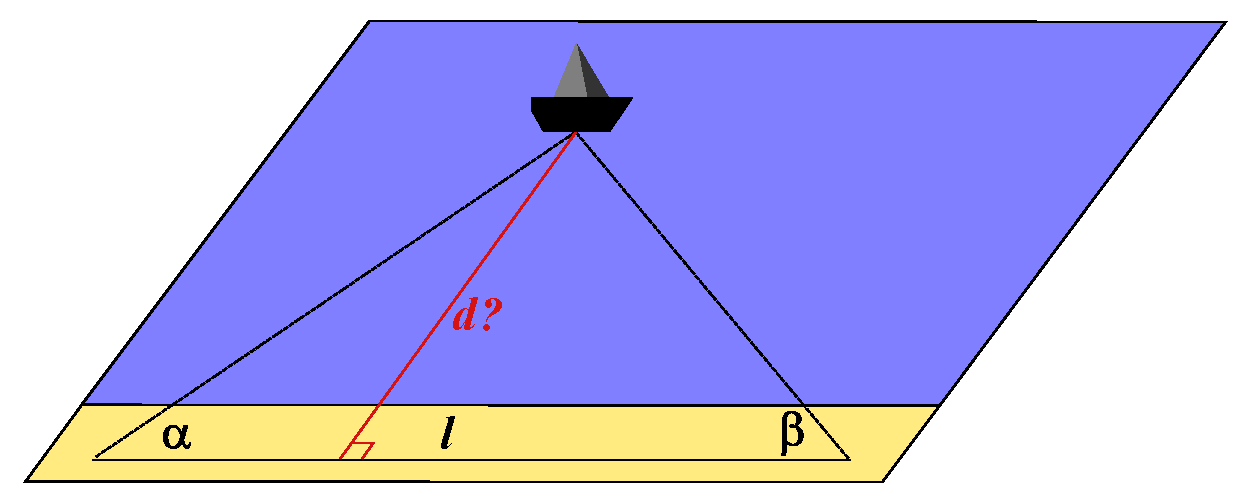
\includegraphics[width=0.67\textwidth]{triangulation}
	\caption{Triangulation. By knowing $\alpha$, $\beta$ and $l$ beforehand, the distance $d$ from the ``ship'' to the side of length $l$ can be calculated using the sine formula (or law of sines) \cite{wiki:triangulation}.}
	\label{fig:triangulation}
\end{figure}

\begin{description}
	\item[Magnetic positioning] is a technique that uses data from smartphone's magnetic sensor, the compass. Most buildings nowadays use reinforced concrete (concrete with steel bars as a skeleton, see \cref{fig:reinforced-concrete}). These bars affect Earth's magnetic field in a unique way \cite{Haverinen:magnetic}. Crowd sourcing may be used to map a building and, later, these maps may be used to locate a device indoors. This technique gives accuracy of 1--2 meters with confidence level of 90\%. However, it is not really that perfect, as the measurement is heavily impacted by moving metal objects inside the building such as elevators, drawer cabinets etc.
	
	\begin{figure}[h]
		\centering
		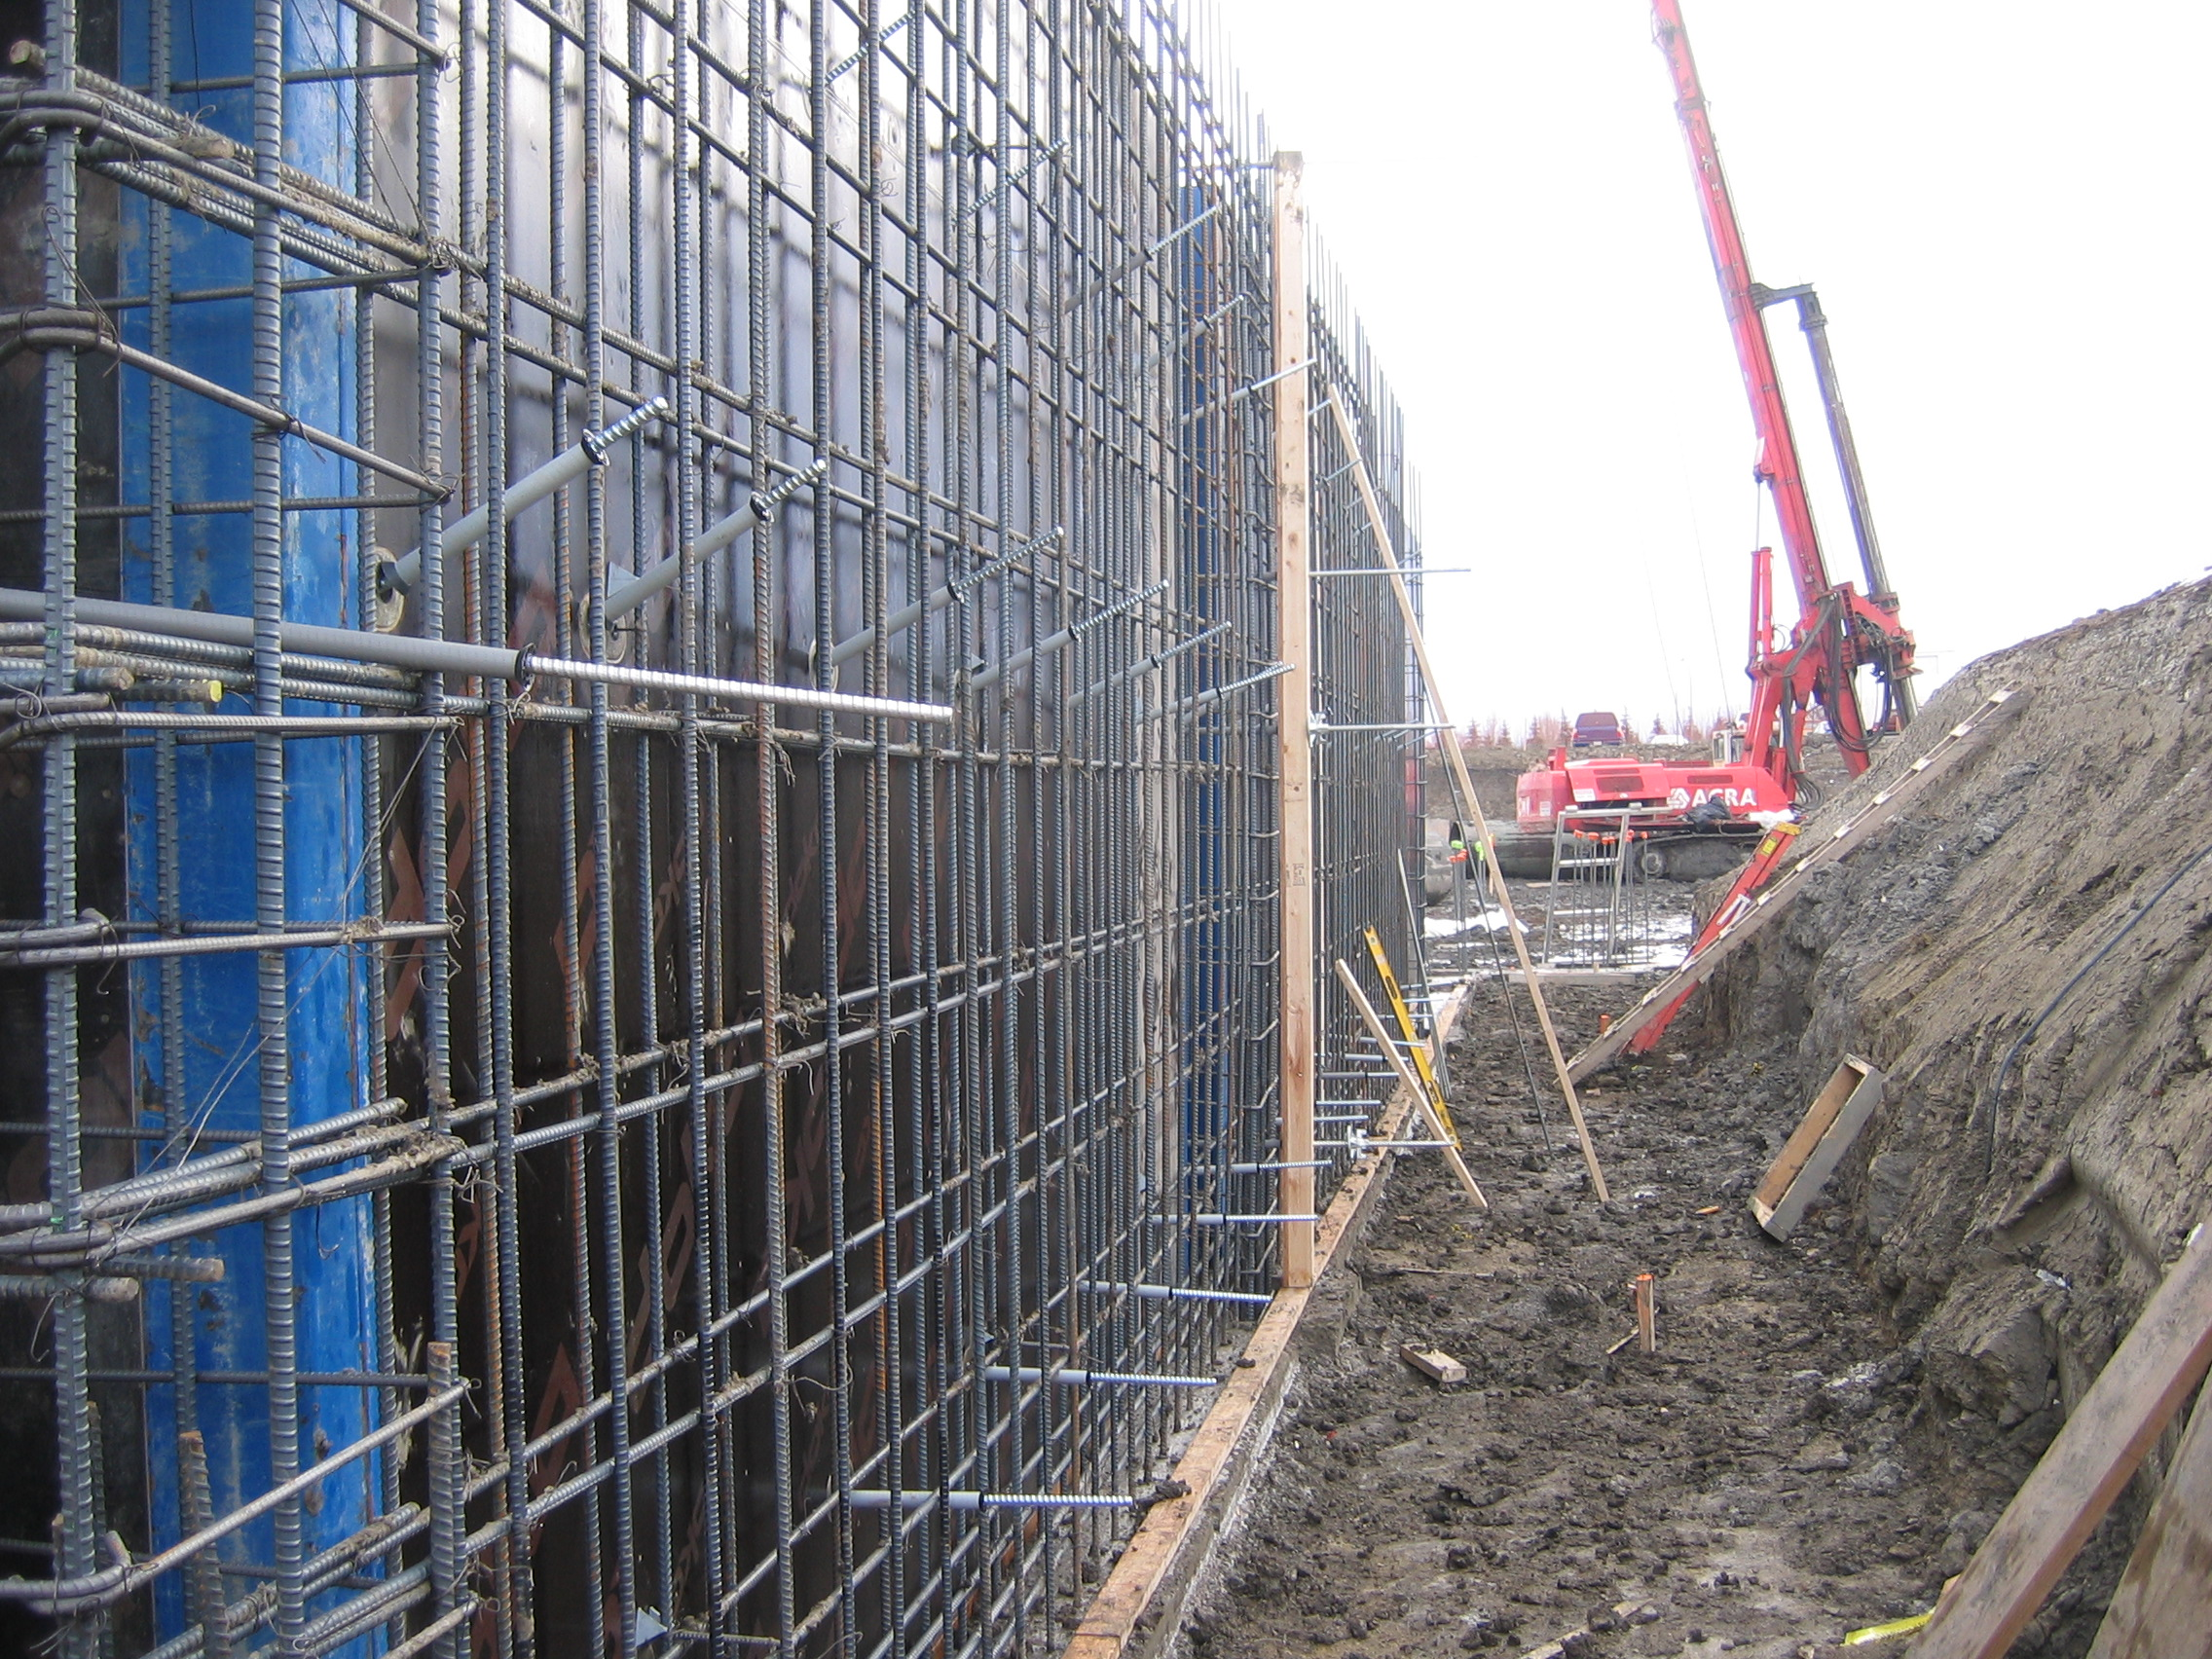
\includegraphics[width=0.67\textwidth]{reinforced-concrete}
		\caption{Steel bar construction prepared for turning into reinforced concrete (still, before pouring the concrete) \cite{penco:concrete}.}
		\label{fig:reinforced-concrete}
	\end{figure}
	
	\item[Inertial measurements] is a pedestrian \emph{dead reckoning} technique and as such is a subject to cumulative errors (among others). When used in a smartphone, built-in sensors---accelerometers in all three axes---provide data from which distinct human steps in time and space can be inferred (see \cref{fig:inertial-measurements}). Later, these steps are overlaid with maps that had to be previously created and user's location is guessed. Even the smallest error made early in this dead reckoning process will manifest itself in every following result, as position $i+1$ is position $i$ with data about $i$-th step added to it. Accelerometers are also pretty noticeable when it comes to battery performance. A lot more energy is being consumed when these sensors are on. Having all these three disadvantages in mind---cumulative errors, battery life and inability to automatically map a previously unknown environment---this is one of the chosen techniques used in physics-based module that provides alternatives for mediation method described in this work (see more about the module in \cref{sec:physics-module}).
	
	\begin{figure}[h]
		\centering
		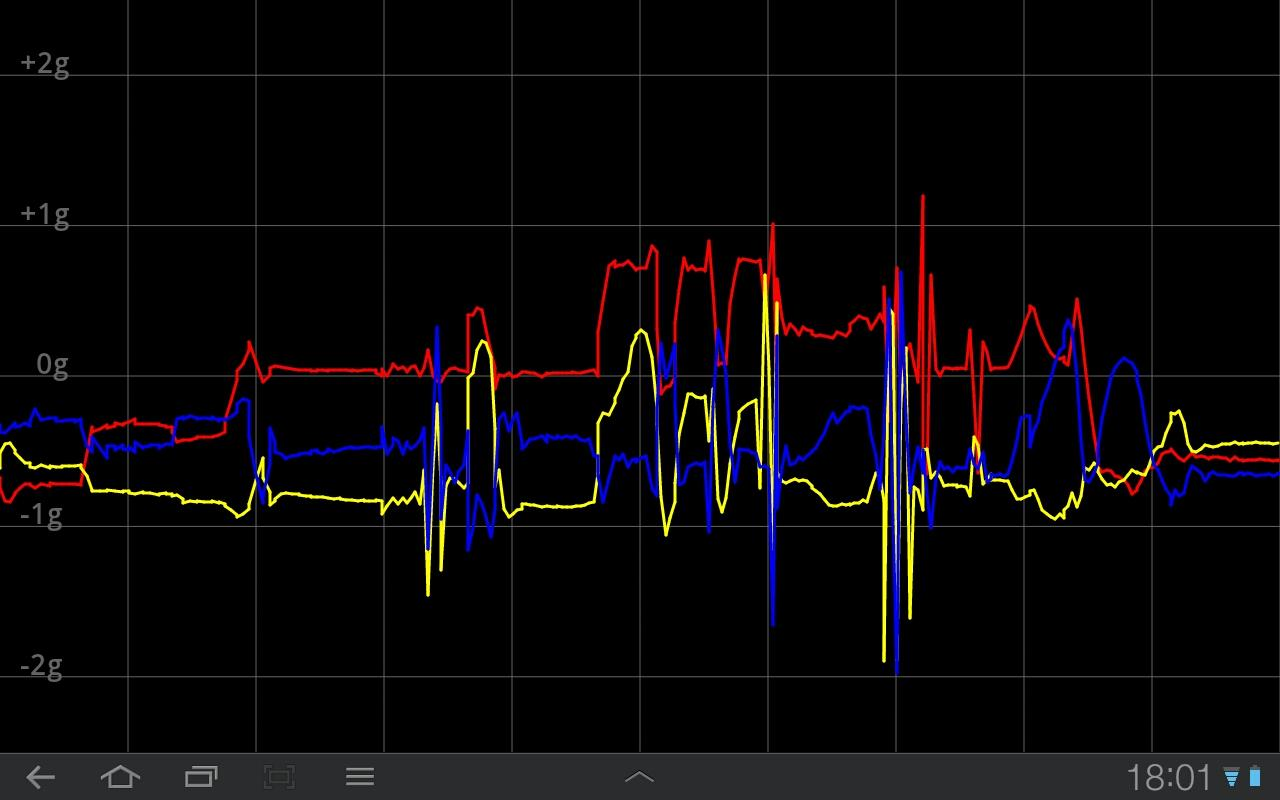
\includegraphics[width=0.67\textwidth]{inertial-measurements}
		\caption{Screenshot of an Android application plotting sensory data from accelerometers in all three axes in real time \cite{google-play:accelerometer}. Some steps can even be seen with the naked eye (the steep fragments).}
		\label{fig:inertial-measurements}
	\end{figure}
	
	\item[Wi-Fi-based positioning] uses information about signal strengths of all visible Wi-Fi networks at a given moment (see \cref{fig:wifi-positioning}). From these strengths, using the Received Signal Strength Indication, we can infer distances to all visible access points. Positions of these are known from a previously prepared map. Using these positions and distances, user's location may be easily obtained. Again, it is possible for signal fluctuation to influence the correctness of this method. One notable realization of this method is ``Anyplace'' from researchers at the University of Cyprus \cite{Anyplace}.
	
	\begin{figure}[h]
		\centering
		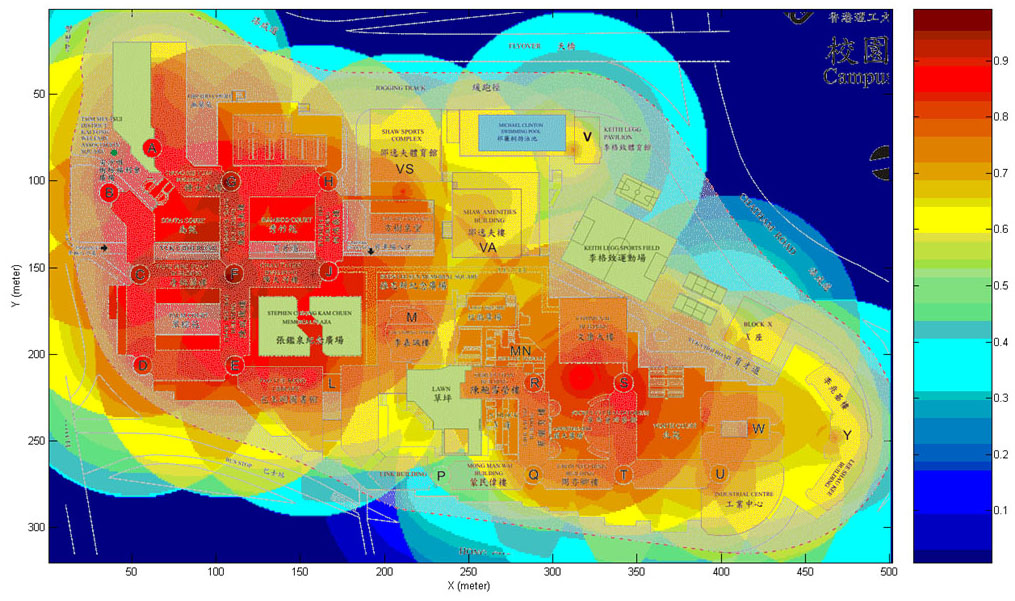
\includegraphics[width=0.67\textwidth]{wifi-positioning}
		\caption{A heat map of Wi-Fi signal strengths at the Hong Kong Polytechnic University \cite{hk:wifi-positioning}.}
		\label{fig:wifi-positioning}
	\end{figure}
	
	\item[iBeacons (via Bluetooth)] are small devices using Bluetooth LE (Low Energy) technology standardized by Apple in 2013. These devices constantly broadcast their unique identifiers to all nearby devices. UUIDs are simply 128-bit numbers usually notated in hexadecimal format, e.g. \texttt{e16d9b56-4d95-48f6-959b-4c8bf701bc6f}. Because of using LE, usually only devices in the same room as the transmitting beacon can receive the signal and by that know what room they're in. Obviously, one has to previously map UUIDs to rooms. Also, not all smartphones currently in use support Low Energy variant of Bluetooth, and thus not all are compatible. Another advantage of using Low Energy variant of Bluetooth  This technique is also used as one of the sources in the physics module (\cref{sec:physics-module}).
	
	\item[RFID] is an acronym for radio-frequency identification. This method is similar in its concept to iBeacons. Small chips with unique identifiers are placed in the room (see \cref{fig:rfid} for some examples of such chips). RFID reader knows the mapping between chips' IDs and rooms/positions. When an ID is read, its matching room is chosen as the user's current location. One big disqualifying disadvantage is that today mobile phones are not RFID readers.
	
	\begin{figure}[h]
		\centering
		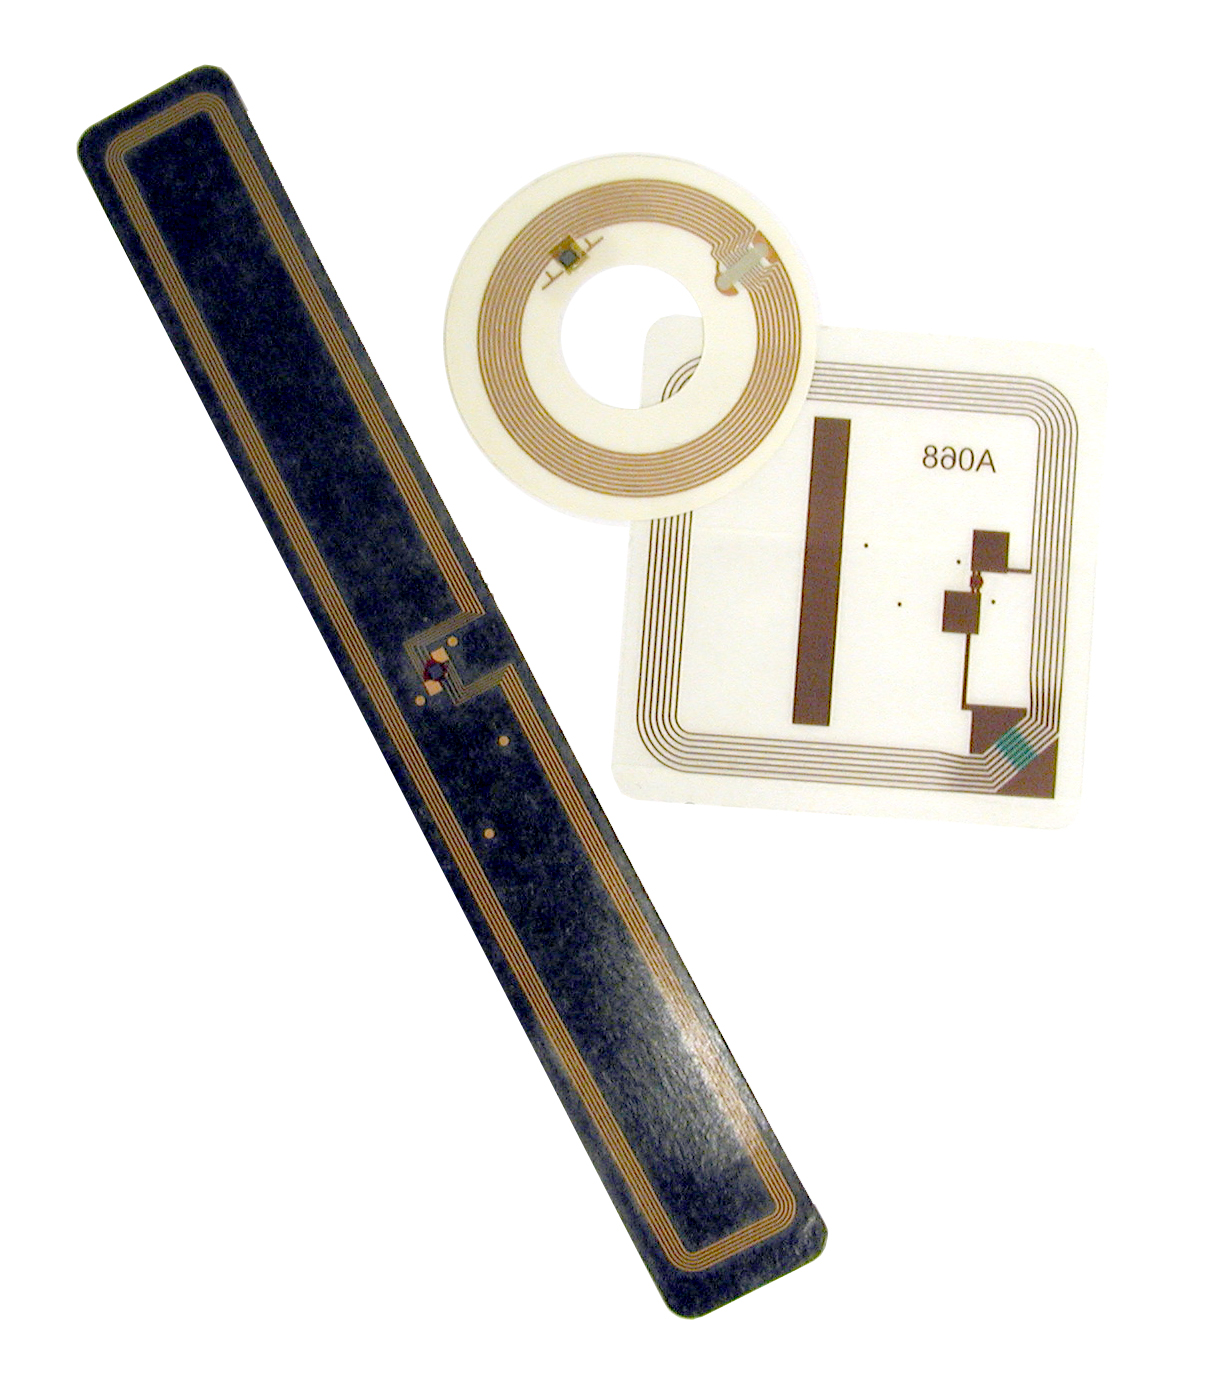
\includegraphics[width=0.5\textwidth]{rfid}
		\caption{Examples of RFID chips used for tagging items and locations \cite{wiki:rfid}.}
		\label{fig:rfid}
	\end{figure}
	
	\item[Grid concepts] revert the receiver and transmitter roles. A device being micro-located broadcasts its identification information, usually by using RFID technology. A large number of receivers are arranged in a grid pattern over an area under observation. Low energy of the signal guarantees that only the receivers closest to the transmitting chip will get its identification. Because of these considerations this method is not readily available for today mobile phones.
	
	\item[Angle of arrival] methods usually need to operate on an array of antennas. Each sensor in the array gets the signal at slightly different time (see \cref{fig:cross-corr-pulse} for a method of calculating this difference). From this time difference of arrival---or TDOA---for the whole array, the angle of arrival can be calculated. Other solutions use highly directional receivers arrange in a circular pattern. A receiver that gets the signal, determines the angle. After having the angle measured for at least 2 distinct transmitters, in the next step, the angles are used during triangulation (\cref{fig:triangulation}) which, in the end, provides array's position.
	
	\begin{figure}[h]
		\centering
		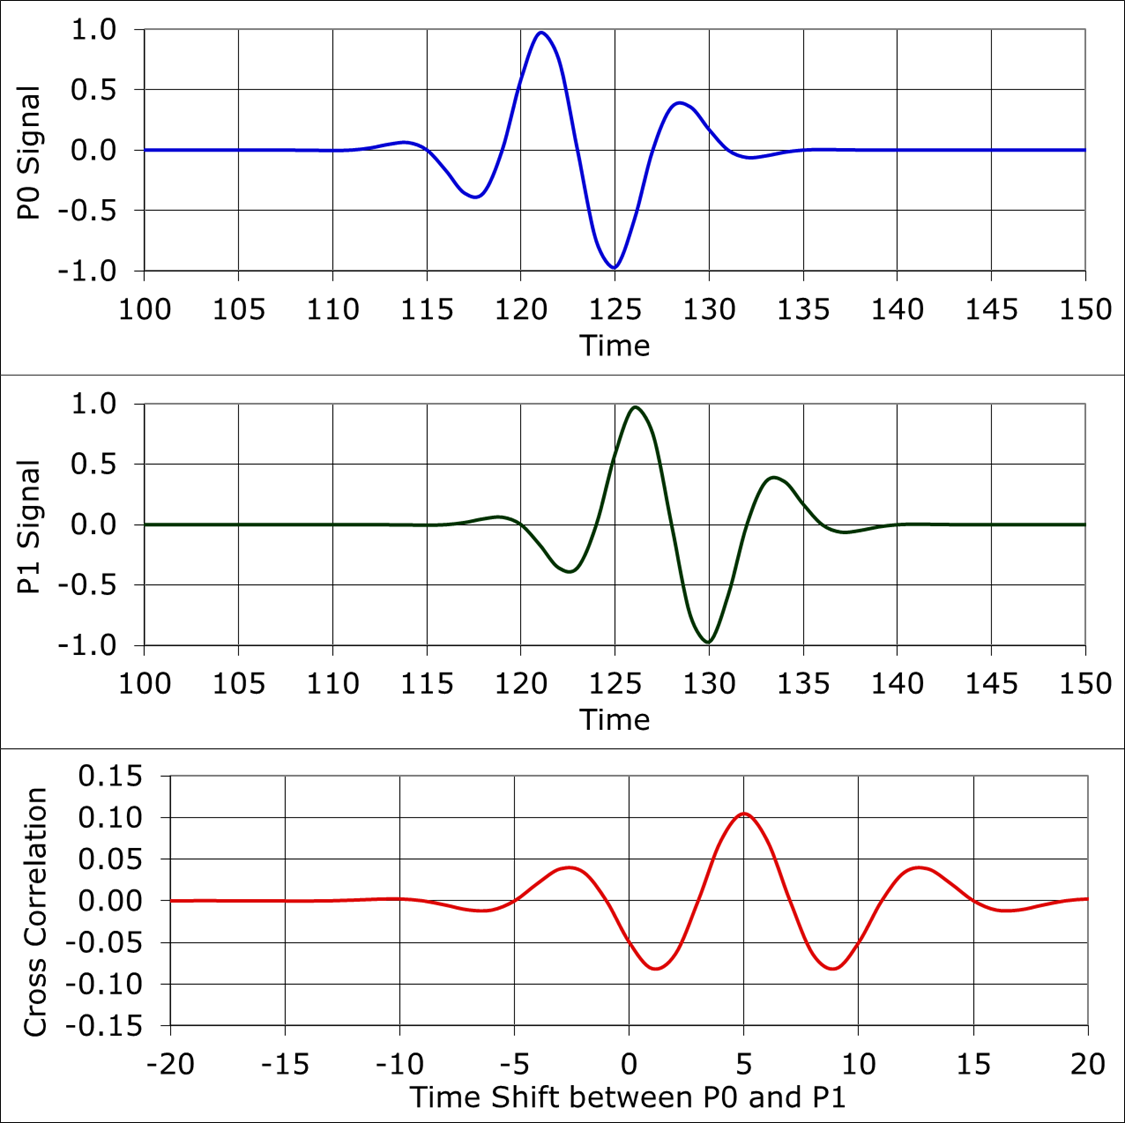
\includegraphics[width=0.67\textwidth]{cross-corr-pulse}
		\caption{Cross correlation between two upper signals shown as the third signal \cite{wiki:cross-corr-pulse}. Maximum in $t=5$ suggests that the signals are shifted by $5$ time units.}
		\label{fig:cross-corr-pulse}
	\end{figure}
	
	\item[Time of arrival] method is slightly similar to \emph{angle} of arrival. When time the signal took to get from a transmitter to a receiver is known, and so is its propagation speed, the traveled distance can be calculated straightforwardly. Transmitted signal has to encode some kind of a time marker, marking the time of sending. The main instantly visible problem here is\ldots extremely accurate time synchronization needed between the both parties. This technique is used in GPS, which is the reason for it being able to be used as a time source.
	
	\item[Ultra-wideband] (also called UWB) is radio transmission method that uses a wide part of the radio frequency spectrum and extremely low energy to transmit large amounts of data over very short distances \cite{ultra-wideband}. These short distances are of interest here, as we don't want to receive signals from other rooms. Unfortunately, modern smartphones are not compatible with this radio technology.
	
	\item[Infrared] communication requires that receivers and transmitters ``see'' each other. Thanks to that, locating based on infrared light would be confined to a single room, a desirable trait. Infrared sensors used to be popular in mobile phones, but this popularity decreased dramatically with the advent of smartphones. Nowadays, it's usable only in custom deployments.
	
	\item[Visible light communication] method is similar in its concept to the infrared-based one. One major difference is that all smartphones have visible light sensors built in, the camera. Zhang and Kavehrad propose a method for indoor localization system based on visible light LEDs \cite{Zhang:visible-light}. Its computer model is able to localize a device in two dimensions with accuracy of centimeters for a reasonably sized room. Along with localization using local warps of Earth's magnetic field, this method is one of the most promising ones. One blatant downside would be the need to lay out the diodes in all rooms being observed, while magnetic positioning works almost out-of-the-box.
	
	\item[Ultrasound] positioning offer much greater accuracy due to the fact that sound travels through air at a \emph{lot} slower speeds than light or other electromagnetic signals. The method works---similarly to RFID positioning---by having simple tags attached to to-be-located objects transmit ultrasound identifying information. Again, such a method cannot be used with currently marketed mobile devices, as these lack capabilities of projecting ultrasonic---in this case---signals with their unique IDs.
	
	\item[QR codes] (abbreviation for Quick Response codes) is a trade name for a particular type of two-dimensional barcode (see \cref{fig:qr-code} for an example of such a code). This method of micro-location is \emph{similarly burdensome and awkward} for the user as the method proposed in this paper (more about bad User Experience in \cref{sec:user-experience}). It works by---first---having these graphical codes laid out in the observed building. Each of them is encoding either a unique identifier of the exact spot it's placed at or even just information about that location directly. Next, the user has to scan a code---take a picture, basically, and then wait for its processing---if they want to learn where exactly this code is physically placed (i.e. just read off information encoded in the QR). Downsides: a lot of preparation needed on the side of the building's management and a lot of awkward hassle for the user. It's worth noting that there exists an Internet movement among software developers aimed at discouraging QR code use to the point of total elimination from public space \cite{should-i-use-qr}.
	
	\begin{figure}
		\centering
		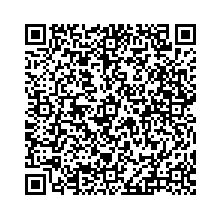
\includegraphics{qr-code}
		\caption{Sample QR-code, version 10 \cite{wiki:qr-code}.}
		\label{fig:qr-code}
	\end{figure}
	
	\item[NFC] is an abbreviation for Near Field Communication. NFC allows enabled devices to establish a radio connection over a very close range (less than 10 cm). This necessary closeness can be used to locate a device with confidence, as the user has to almost touch a tag with their device (so they have to be near it), to read it. At the same time this requirement renders this method highly impractical and burdensome for the user. The NFC technology is only built into new smartphones by Apple and most premium Android phones, and because of that it is not compatible with most devices currently in use. These points don't stop some researchers from publishing a paper about their proposed framework for such a micro-location method \cite{nfc-ulocation}. As a tidbit, this is also the technology used in contactless payments using credit and debit cards.
	
\end{description}

\section{Mediation. The proposed method}
\label{sec:mediation}

\todo[inline]{Motivation for using semantic maps}
